
\noindent\textbf{Simulations}
%
Despite large amounts of noise introduced into the simulated measurements, and
the missing observations, both the Kalman filter and smoother yielded accurate
estimates of true positions.
%
The Kalman filter and smoother provided more accurate estimates of velocities
and accelerations than the baseline finite differences method.
%
We also obtained more accurate estimates with learned than with manually set
parameters.
%
Specially for missing observations, estimates by the Kalman smoother were more
accurate than those by the Kalman filter.

\noindent\textbf{Mouse tracking}
%
The interactive figure shows positions extracted with the computer vision
functions and those inferred by the Kalman filter and smoother, for an example
session. At time with missing observations (i.e., missing black dots) the
Kalman smoother provided more natural position estimates than the Kalman
filter, that sometimes went astray.
% 
As with simulated data, estimates of velocities and acceleration by the
baseline finite differences method appeared noisy, and those from the Kalman
filter and smoother seemed less noisy (data not shown). Extrapolating from the
simulation results, we infer that, also for the mice tracking, Kalman filter
and smoother velocity and acceleration estimates were more accurate than those
from the finite difference method.

\begin{figure}
    \begin{center}

        \href{http://www.gatsby.ucl.ac.uk/~rapela/fwg/reports/learning/figures/positions_smoothed_session003_start0.00_end15548.27_startPosition0_numPosition10000_pos_learnedParams.html}{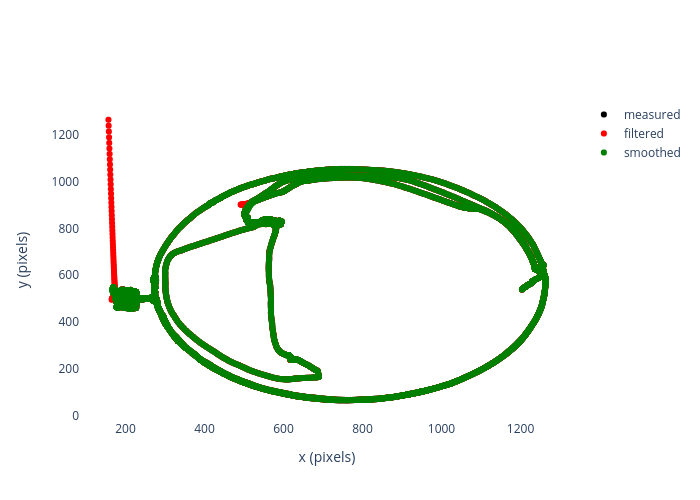
\includegraphics[width=3in]{figures/positions_smoothed_session003_start0.00_end15548.27_startPosition0_numPosition10000_pos_learnedParams.png}}

        \caption{Positions measured with the computer vision functions (black)
        and Kalman filtered (red) and smoothed (green) positions from a LDS
        model with learned parameters. Click on the figure to access its
        interactive version, and double click on a trace legend to hide/show
        the trace.}

    \end{center}
\end{figure}

